\chapter{Deformation studies of a ladder under the test beam}

  The first full-scale prototype which embeds twelve sensors glued on a copper flex-cable and a 8 \% density \gls{SiC} foam was tested in November 2011 at CERN-SPS facility with a pions beam of 120 GeV.
  The motivations to perform such a test in real conditions are to, firstly, make sure that the ladder is working properly.
  Secondly, to verify the response homogeneity of each sensor.
  Finally, it has to prove the benefits of a double sided measurement.
  This chapter does not aim to present fully the test beam campaign and all the results, but to focus on a specific study of the ladder's deformation observed during the alignment procedure.
  More results about this test beam is presented in Loic Cousin's thesis\cite{cousin}.
  This chapter will present the test beam facility, as well as the experimental set-up.
  The alignment procedure is explained and some results for the ladder positioned in a normal incidence, as well as the ladder titled in one direction are discussed.
  The second part of the sensor will focus on the deviation observed during the alignment and will discuss a method to overcome these deformations.
  Finally, the benefits of double-sided measurements will be introduced.
  
  \minitoc

  \section{Test beam of the full complete PLUME ladder at CERN}

    \subsection{Test beam facility and beam test set-up}

    The test beam was performed at CERN-SPS in the North hall on the H6 beam line.
    Negative pions with an energy of 120 GeV were used.
    The spill structure is 9.6 s with a dead time of 45.6 s. 
    The bench set-up is composed of a telescope made of four standard MIMOSA-26 sensors, thinned down to 120 $\mu\text{m}$ and used as reference planes.
    The telescope is made of two arms, with a distance between the two sensors of the same arm of 5 mm.
    The reference planes are stabilised to a temperature of 15 degrees Celsius and a 8 sigma S/N threshold cut was applied.
    In the middle of the two arms, the PLUME ladder is placed and for the following of the chapter it is denominated as the \gls{DUT}.
    The bench has also $7 \times 7$ scintillators used for triggering the data.
    Most of the runs were taken with a trigger frequency between 2 and 8 kHz, except for two days where the frequency was oscillating between 1 and 1.3 kHz.
    The acquisition system is limited to eight inputs and four inputs are used by the telescope.
    Thus, only four sensors of the \gls{DUT} were connected to the acquisition, two on each side.
    The temperature of the \gls{DUT} was stabilised thanks to air flow cooling system, provided by a fan.

    %The bench set-up is composed of 4 standards 120 $\mu\text{m}$ thinned MIMOSA-26 used as telescope planes, the PLUME ladder, called here \gls{DUT} and a $7 \times 7 \text{mm}^2$ used for triggering. 
    %The reference planes are at 8 sigma S/N cut and stabilized to a temperature of 15 degrees Celsius.
   % The telescope is made of two arms, on each side of the \gls{DUT} and the distance between two sensors of the same arm is 5 mm.
    %Nonetheless, for one experimentation, the telescope was set-up differently, as discussed later.
    %Most of the runs were taken with a trigger frequency between 2 and 8 kHz except for two days on which it was between 1 and 1.3 kHz.
    %As the acquisition system is limited to eight inputs and the set-up has four reference planes, only four sensors of the \gls{DUT} were connected, two on each side.
    %Nevertheless, due to the size of the scintillator, the acquisition of sensors outside the beam is not mandatory. 
    %Thus, it reduces the data band-with.
    %Two different air flow speeds were used: 3 $\text{m.s}^{-1}$ and 6 $\text{m.s}^{-1}$. 

    \subsection{Cartesian coordinate systems}

    Although the sensors have their own ID to distinguish them during the analysis, the position of each plane has to be known exactly.
    Two Cartesian coordinate systems are then defined.
    The first one is the global one and is determined by the position of each sensors of the telescope.
    The notation used for this coordinate system is $(x,y,z)$.
    The $x$-axis corresponds to the horizontal direction, the $y$-axis is the vertical one and the $z$-axis is along the beam direction.
    The origin $(0,0,0)$ of the system is defined with respect to the center of the two reference planes arms.
    The second coordinate system is the local one and is determined for a single sensor.
    To differentiate this reference the $(u,v,w)$ notation is used.
    The $u$-axis corresponds to the pixel rows, the $v$-axis is along the pixel columns and the $w$-axis is perpendicular to the matrix.
    The origin of the local system is the center of the pixel matrix.
    The figure~\ref{fig:labCoordinates} summarises the definition of the two coordinate systems.

    \begin{figure}
      \centering
      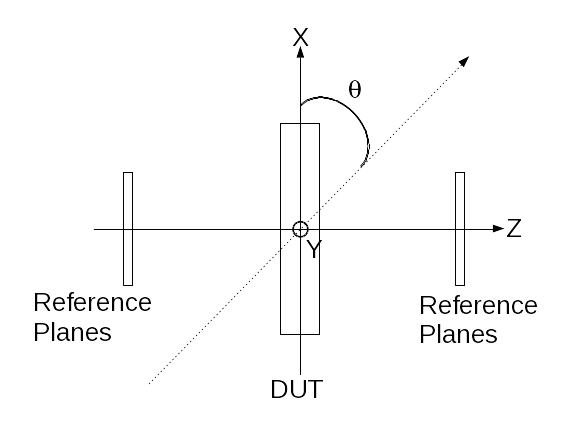
\includegraphics[width = 0.7\textwidth]{Pictures/deformation/lab_frame.png}
      \caption{Drawing of the laboratory coordinates.}
      \label{fig:labCoordinates}
    \end{figure}

    \subsection{Measurements}

    The prototype validation was done under several conditions.
    Firstly, three different geometric configurations were used.
    On the first one presented on the figure~\ref{fig:tbNormal}, the \gls{DUT} is parallel to the telescope planes and the beam is hitting the device in a normal incidence.
    The \gls{DUT} is placed in between the two arms, with the middle in a center of the foam.
    For the second configuration, as shown on the figure~\ref{fig:tilt36}, the distance between the telescope planes are the same, but the \gls{DUT} is tilted between 28 and 40 degrees along the $y$-axis.
    Runs with a larger angle (60 degrees) were done.
    Due to the PLUME box's size, the cabling for the acquisition, the air cooling system and the design of the telescope stage, limiting the spacing between the two arms, the \gls{DUT} was placed behind the two arms, as presented on the figure~\ref{fig:tilt60}.
    For both configurations, different parameters were modified.
    The thresholds were set to 5 and 6 mV, different sensors were aimed and the air flow speed was set to 3 $\text{m.s}^{-1}$ and 6 $\text{m.s}^{-1}$.

    \begin{figure}[!h]
      \centering
      \begin{subfigure}[t]{0.9\textwidth}
        \centering
        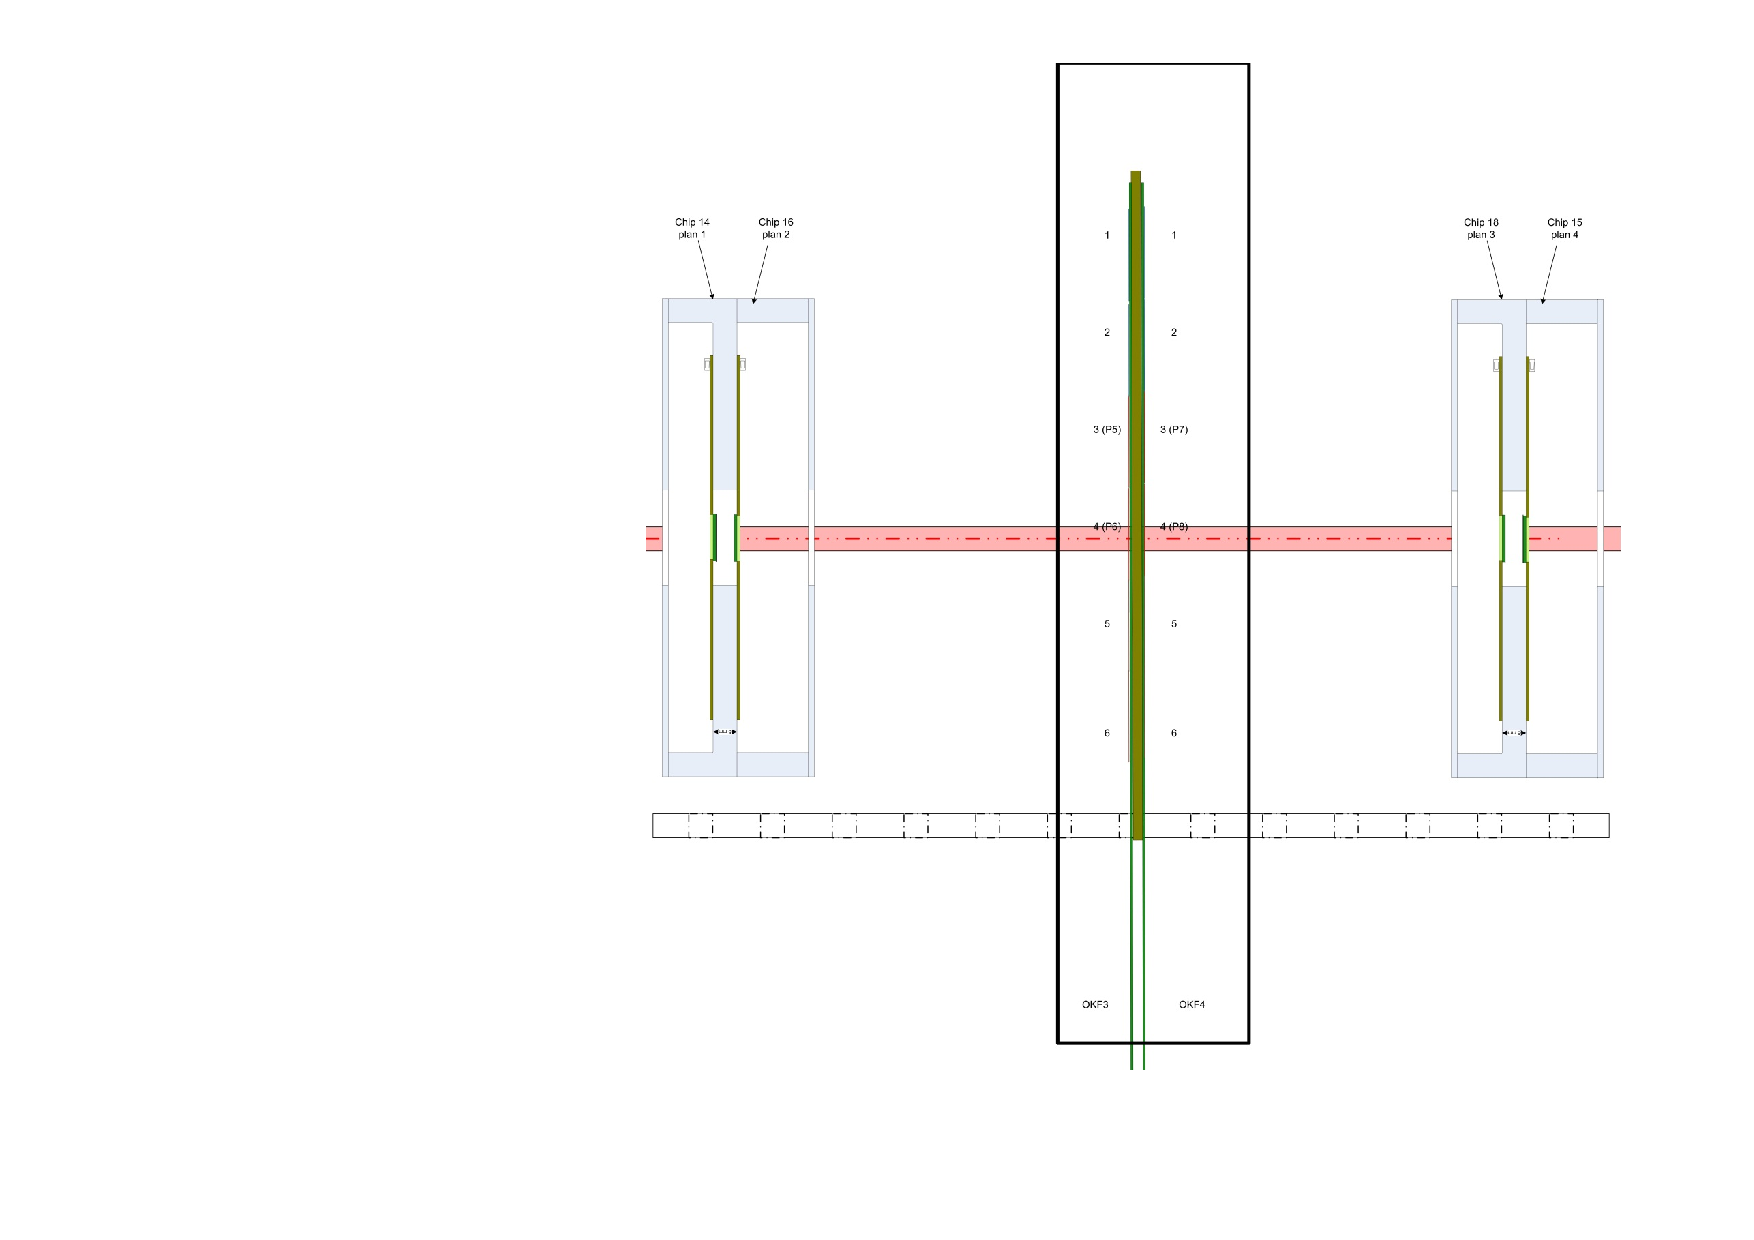
\includegraphics[width = 0.5 \textwidth]{Pictures/deformation/tb_cern_11_sketch_normal.pdf}
        \caption{Set-up for the PLUME ladder in normal incidence with respect to the beam direction.}
        \label{fig:tbNormal}
      \end{subfigure}

      \begin{subfigure}[t]{0.45\textwidth}
        \centering
        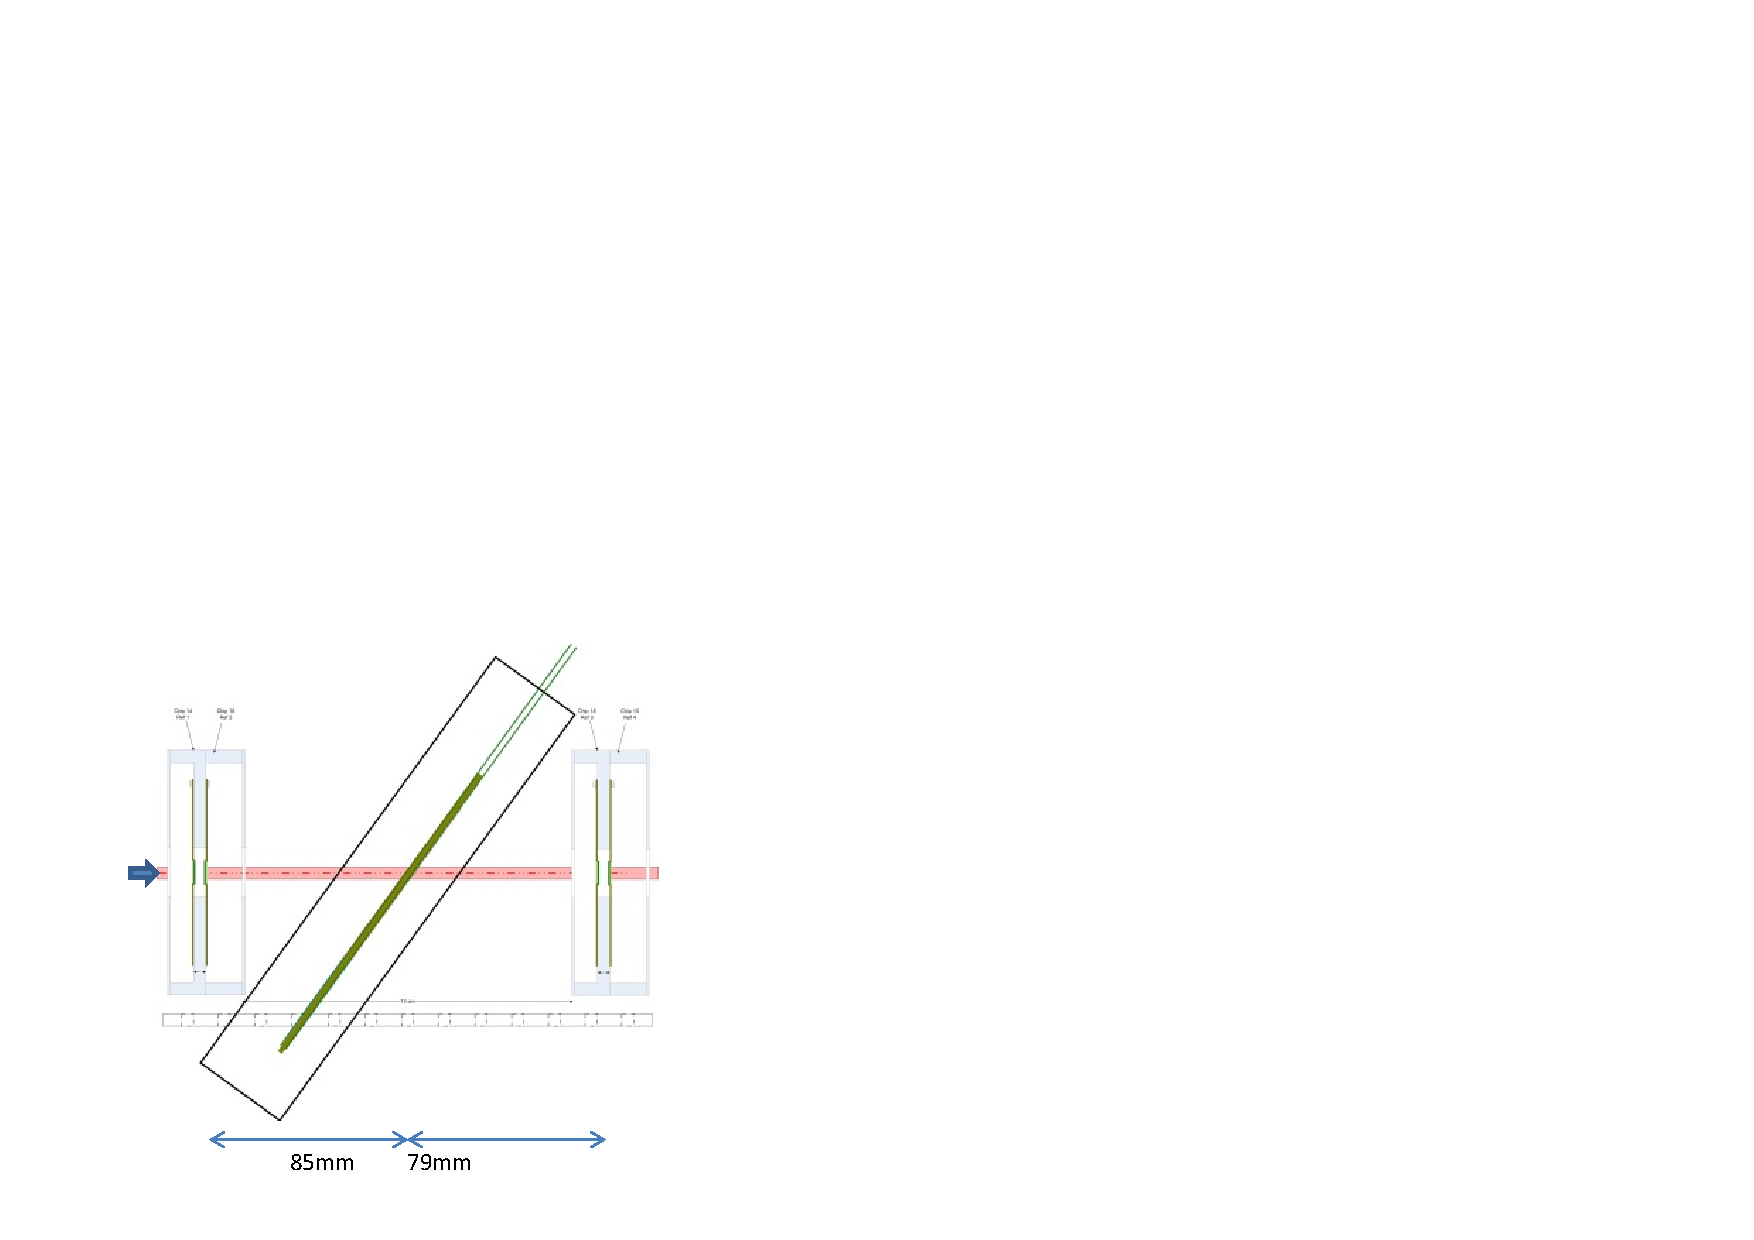
\includegraphics[width=0.8\textwidth]{Pictures/deformation/tb_cern_11_sketch_tilted.pdf}
        \caption{Configuration for an angle between 28 and 40 degrees.}
        \label{fig:tilt36}
      \end{subfigure}
      ~%\quad
       %add desired spacing between images, e. g. ~, \quad, \qquad, \hfill etc. 
        %(or a blank line to force the subfigure onto a new line)
      \begin{subfigure}[t]{0.45\textwidth}
        \centering
        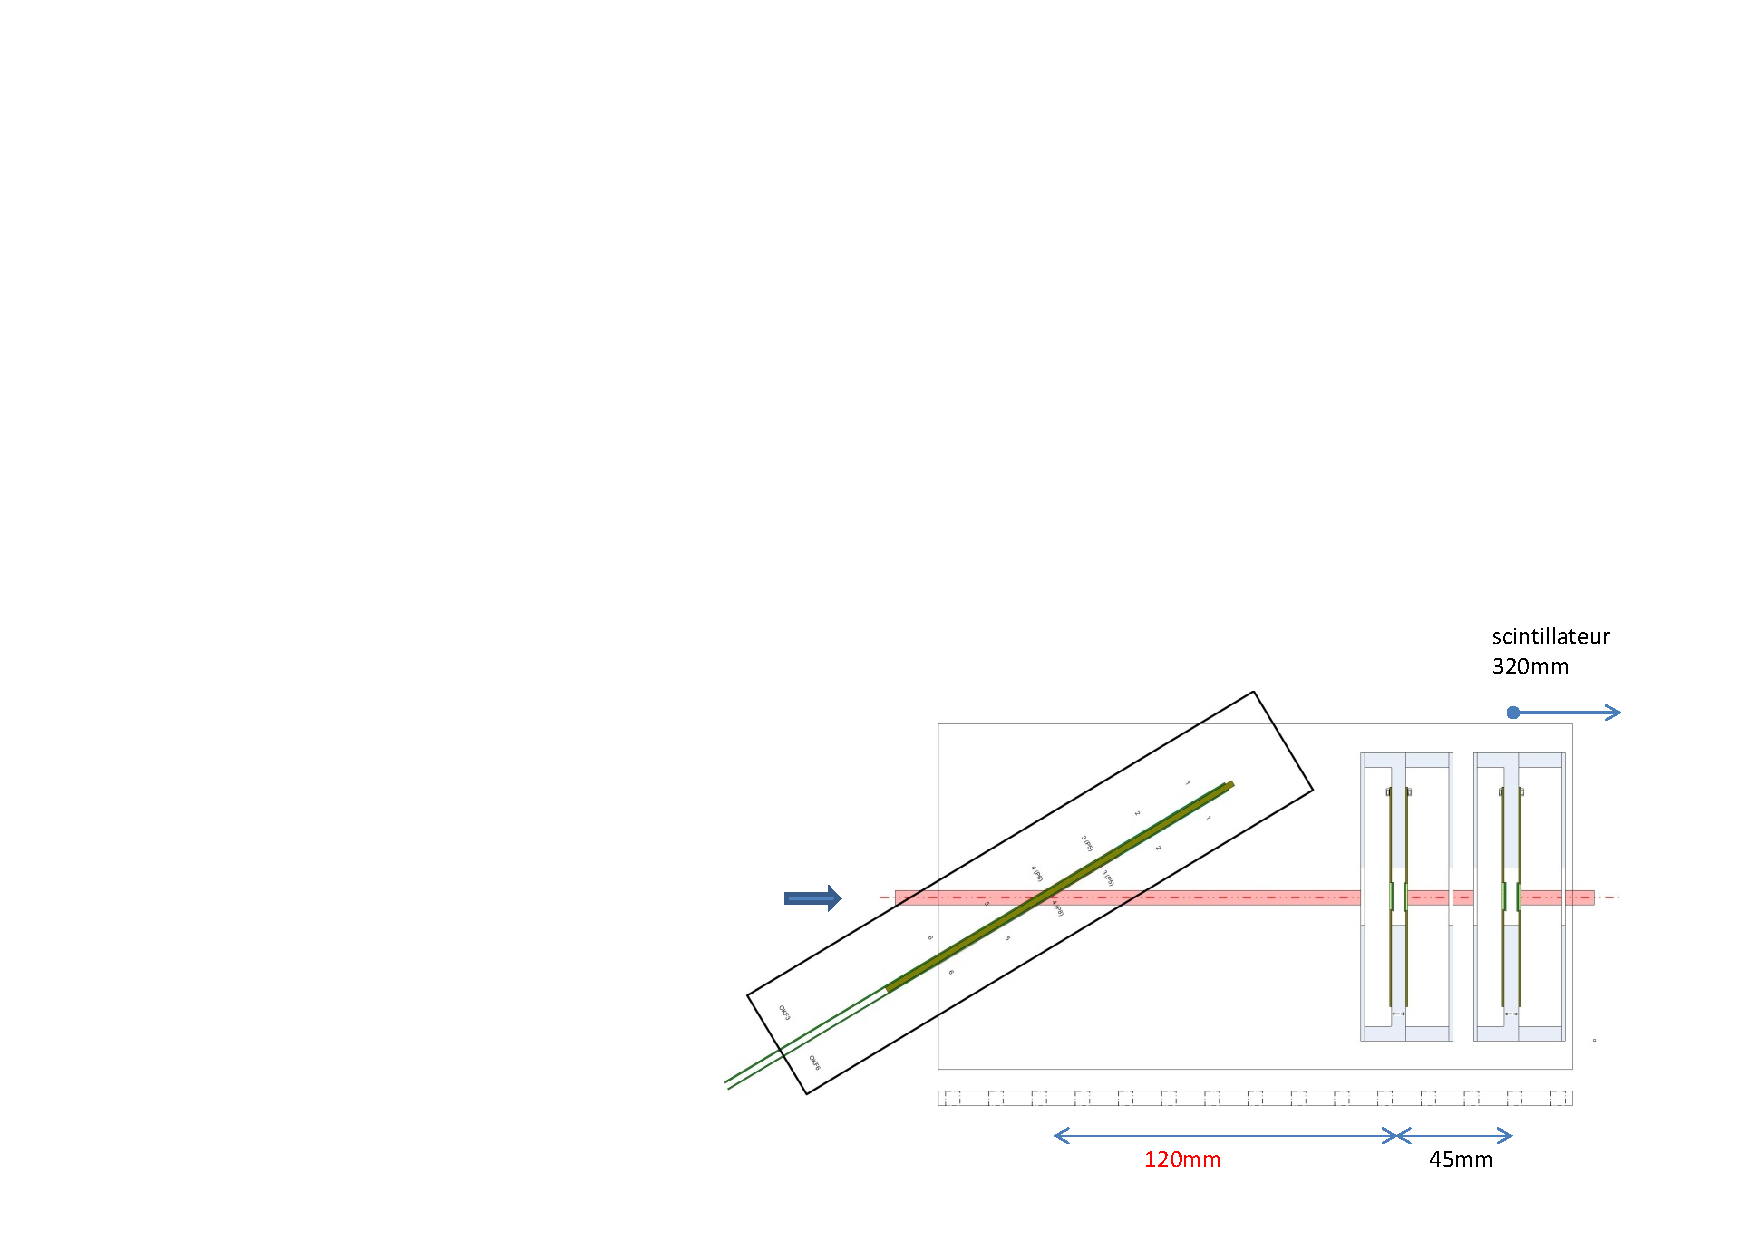
\includegraphics[width=0.95\textwidth]{Pictures/deformation/tb_cern_11_sketch_tilted120mm.pdf}
        \caption{Configuration for an angle of 60 degrees.}
        \label{fig:tilt60}
      \end{subfigure}
      \caption{Top view sketches of the test beam configuration for different ladder positions.}
      \label{fig:tilt}
    \end{figure}   

    The analysis and the results shown in the following sections were performed with \gls{TAF}, the analysis software developed by the IPHC and presented in chapter~\ref{chap:labTests}.

  \section{Spatial resolution studies}
   
    One of the measurement performed during the analysis is to determine the pointing resolution of the ladder.
    As the sensors used are well-known, the performance of the ladder should be similar to the one expected and the mechanical structure should have a small impact.
    Any deviations on the pointing resolution or the efficiency might point out an unexpected impact of this mechanical structure on the whole system.
    %The sensors used are well-known and they should have a pointing resolution similar to the one expected, regardless the mechanical structure.
    %Any deviations might point out an impact of the mechanical structure on the whole system.
    The alignment steps to obtained the pointing resolution of the ladders are explained below for different run configurations. 

    \subsection{Normal incidence track}

    Only the hit position is provided by each sensor.
    To perform an analysis, the telescope planes have to be aligned each other.
    The hit information of every plane are combined in order to create tracks. 
    A track correspond to the path of a particle through the system.
    Thanks to this information, the tracks are then compared to the hit position on the \gls{DUT} to give some information, such as the detection efficiency (the ratio of tracks matched to hits on the \gls{DUT}), the spatial resolution (minimum distance to distinguish two incoming tracks).

    The alignment procedure is done in two steps: firstly the telescope planes are aligned to minimise the mismatch of particles' tracks and to improve the tracking resolution.
    Afterwards, the \gls{DUT} is aligned with respect to the information provided by the reference planes and then, the analysis itself is performed.
    Although the position of each sensors is measured during the test beam with a precision of the millimeter, for the analysis, a precision of the micron level has to be achieved.
    Three degrees of freedom were taken into account for the alignment here: two translations for the $x$ and $y$-axes and one rotation around the $z$-axis.
    The $z$ position is determined by the position measured during the test beam campaign and is not considered as a free parameter due to the beam used.

      \subsubsection{Alignment procedure and telescope alignment}

      Firstly, the data acquired during the test beam are processed to extract the signal and the hit information.
      For each frame, the position of the pixel(s) having a signal above the discriminator threshold is stored and assigned to an ID corresponding to a sensor.
      The analysis software is in charge to assign correctly the hit to the sensors and then to group the pixel fired into clusters.
      As the sensors used during the test beam have a binary output, no information on the seed pixel is provided.
      Thus, the hit position is obtained from a center of gravity calculation.

      Secondly, on the analysis software, one plane is considered as the origin of the telescope coordinate system and is used as a reference for the alignment.
      Usually, the first sensor hit by the beam is the main reference.
      The alignment means to correct the offset for the view angles and the hit position of the telescope planes and the \gls{DUT}.
      These offsets are found thanks to scatter plots where the residuals is represented as a function of predicted hit position.
      An alignment is considered as a good one when the residuals is not correlated to the predicted hit position.
      If it is not centered in zero, an offset has to be applied in this direction, whereas a slope indicates that a tilt has to be applied.
      First off, the hit position of the first plane are extrapolated to the next planes in order to perform the alignment.
      This tracks extrapolated are straight line perpendicular to the hit position.
      Thus, the hit position of the last telescope plane are adjusted to match the hit position of the first plane.
      The alignment is an iterative procedure which consists to minimise the residual. 
      It corresponds to the distance between the extrapolated track to the closest hit on the sensor.
      Afterwards, the track candidates are built by matching a hit on the first plane to a hit on the last one.
      The second and third telescope planes are aligned with respect to the information provided by the extrapolated tracks.
      For example, the figure~\ref{fig:alignmentPlane2} and~\ref{fig:alignmentPlane3} show the residual distributions of the second and third planes in the $u$ and $v$ direction with respect to the tracks built by the first and the last planes.

      \begin{figure}
        \centering
        \begin{subfigure}[t]{0.45\textwidth}
          \centering
          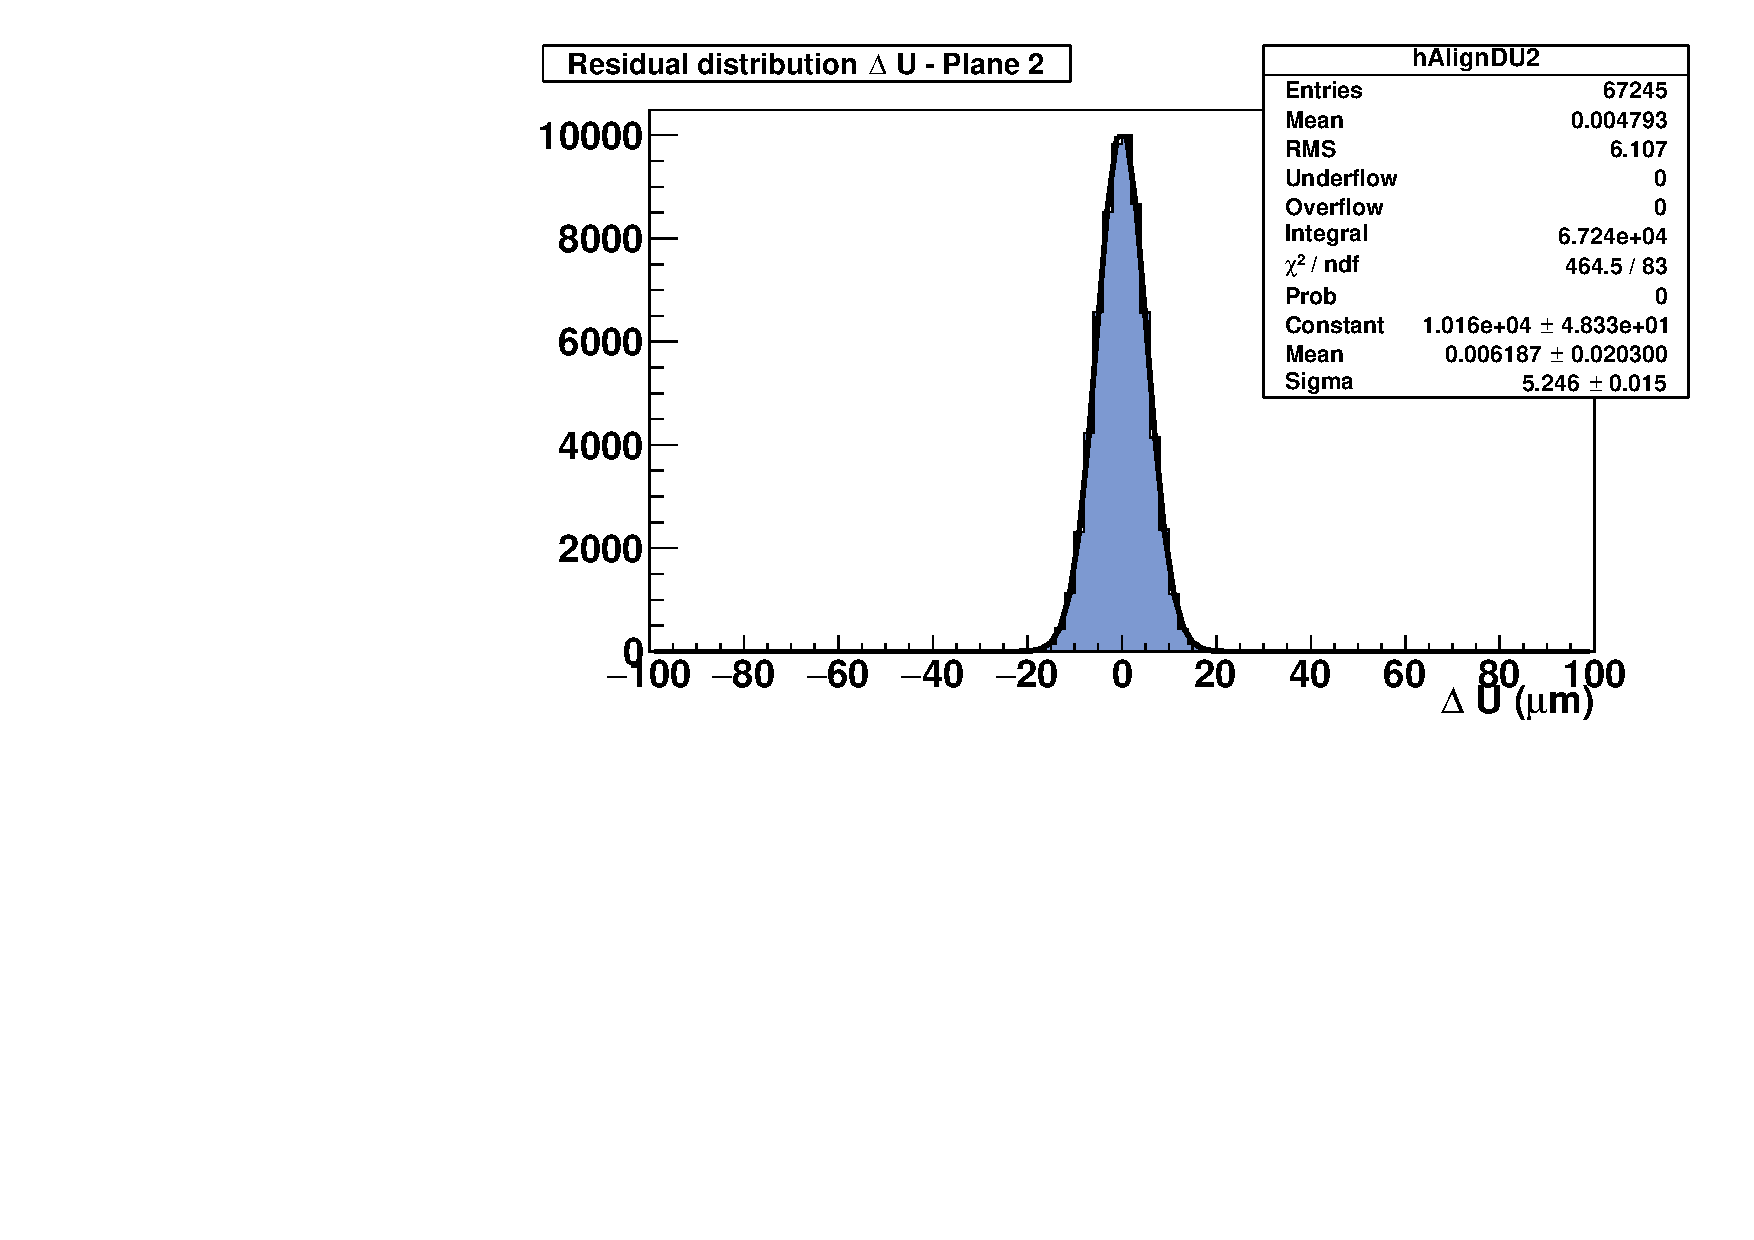
\includegraphics[width = 1.2\textwidth]{Pictures/deformation/residualUPl2_226056.pdf}
          \caption{Along $u$ direction.}
          \label{fig:alignmentPlane2}
        \end{subfigure}
        \hfill
         %add desired spacing between images, e. g. ~, \quad, \qquad, \hfill etc. 
          %(or a blank line to force the subfigure onto a new line)
        \begin{subfigure}[t]{0.45\textwidth}
          \centering
          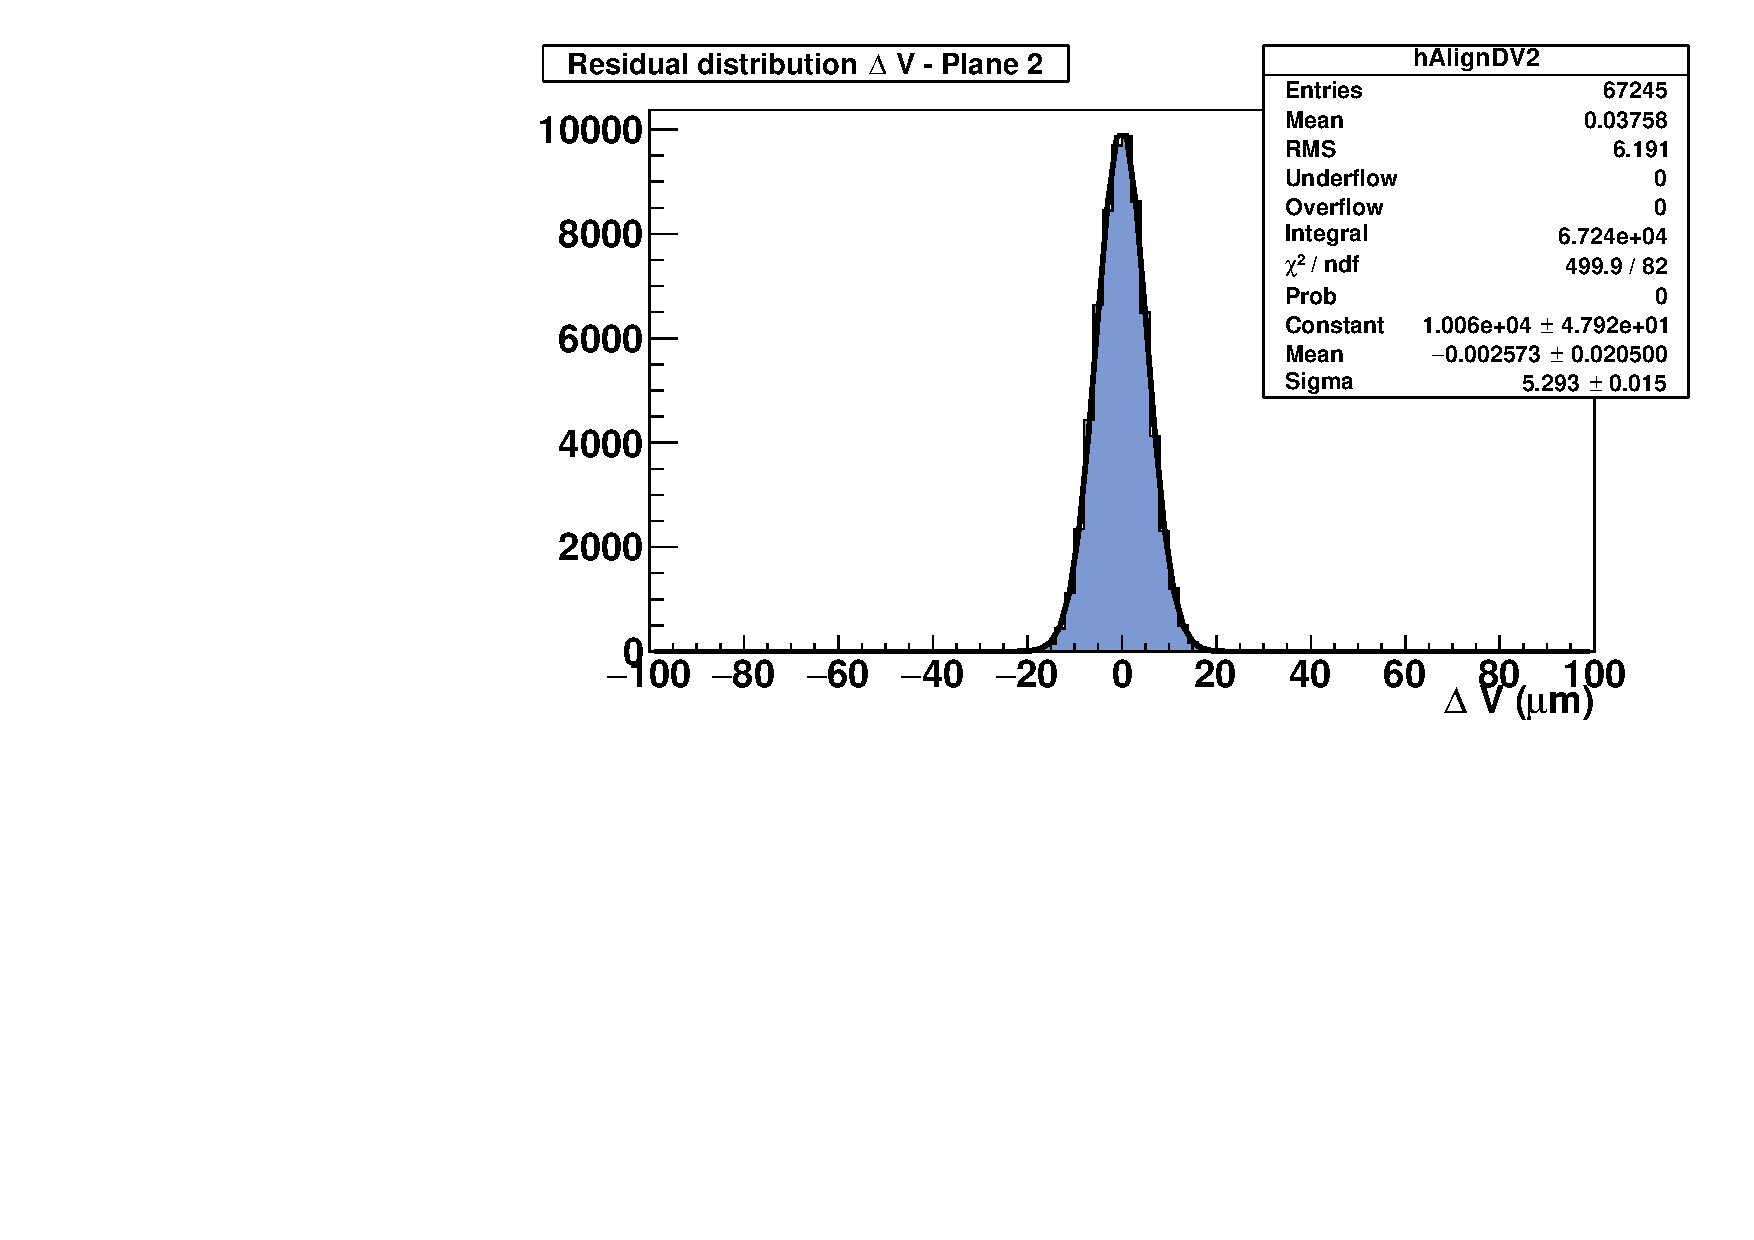
\includegraphics[width = 1.2\textwidth]{Pictures/deformation/residualVPl2_226056.pdf}
          \caption{Along $v$ direction.}
          \label{fig:alignmentPlane3}
        \end{subfigure}
        \caption{Residual distributions in the $u$ and $v$ directions for the middle telescope planes.}
        \label{fig:alignmentTelescope}
      \end{figure}

      As already explained, the alignment is an iterative procedure.
      To find a hit matching a track, a region of interest is defined.
      At the beginning, a hit in a $1000 \times 1000 \text{ }\mu\text{m}$ around the extrapolated one is search.
      Step by step, the region of interest is restricted to achieve a region of six times the pitch.
      
      After the telescope alignment is done, a track candidate is dismissed if it is made of less than four hits or if the $\chi^2$ fit is greater than a fixed value determined by the user. 
      For the alignment, two assumptions are defined. 
      The telescope planes are parallel each other.
      Thus the alignment consists of a translation along $x$ and $y$ and a rotation around the $z$-axis.
      As the test beam was performed without a magnetic field and pions of 120 GeV were used, the Coulomb multiple scattering is neglected.
      So, the tracks are perpendicular to the detectors and the alignment is not sensitive to the $z$ position.
      A precision of the millimeter level for the position does not have a huge impact on the alignment.

      \subsubsection{Alignment of the DUT}

      When the telescope alignment is done, the reference tracks reconstructed by the reference planes are used to align the \gls{DUT}.
      Its $z$ position is fixed, nonetheless, two degrees for freedom are added: the rotations along the $x$ and $y$-axes, plus the three other degrees of freedom defined above.
      To assist the user in the alignment steps, several plots are produced. 
      The figure~\ref{fig:UdeltaU} represents the residual in the $u$ direction as a function of the hit position on the plane in the same direction.
      The residual should not be correlated to the hit position on the plane.
      A slope or an offset indicates respectively a tilt in one direction and a shift in one direction.

      \begin{figure}
        %\centering
        \missingfigure{Delta-U = f(U)}
        \caption{Scatter plot of the residual in the $u$ direction as a function of the hit position on the plane in the same direction.}
        \label{fig:UdeltaU}
      \end{figure}

      \begin{figure}
        %\centering
        \missingfigure{Track-hit residual as a function of the hit position (normal incidence)}
        \caption{Distribution of the residuals for the DUT.}
        \label{fig:alignmentDUT}
      \end{figure}

      The figure~\ref{fig:alignmentDUT} shows the residuals distribution in both direction for one sensor of the \gls{DUT}.

      The resolution measured $\sigma_{Res}$ here is a combination of the resolution of the telescope $\sigma_{tel}$, the multiple scattering $\sigma_{M.S}$ and the pointing resolution of the sensor $\sigma_{DUT}$, as described in equation~\ref{eq:pointingResolution}.
      
      \begin{equation}
        \sigma_{Res}^2 = \sigma_{tel}^2 + \sigma_{DUT}^2 + \sigma_{M.S}^2
        \label{eq:pointingResolution}
      \end{equation}

      As it was already explained, the Coloumb multiple scattering is not significant here.
      Thus, the pointing resolution of a sensor of the \gls{DUT} is then:

      \begin{equation}
        \sigma_{DUT} = \sqrt{\sigma_{tel}^2 - \sigma_{Res}^2}
      \end{equation}

      For the sensors studied here, the spatial resolution achieved is ... $\mu\text{m}$.

    \subsection{Ladder tilted in one direction}

      The same alignment procedure as presented above, was applied for runs where the ladder was tilted with respect to the beam direction, as shown on the figure~\ref{fig:tilt}.
      Nevertheless, the alignment is more complicated.
      
      \begin{figure}
        %\centering
        \missingfigure{Track-hit residual as a function of the hit position (tilt)}
      \end{figure}
    
      \subsubsection{Origin of the deviations}

      The deviations observed here are caused by the characteristics of the ladder.
      Indeed, ultra-thin sensors with a thickness of approximately $50 \text{ }\mu\text{m}$ are used.
      Naturally, without any mechanical structure, the sensors tend to be very flexible.
      Nevertheless, the gluing procedure to the flex-cable and the \gls{SiC} foam induces permanent deformations of the surface of about $10 \text{ }\mu\text{m}$ that can not be flatten.
      Also, the foam has an open-cell structure with small bumps.
      The Bristol group has performed a mechanical survey on a mechanical prototype.
      This prototype has non-functioning MIMOSA-20 sensors that were thinned and attached to the standard flex-circuits.
      The measurements done with an optical survey equipment have revealed a peak-to-peak flatness of the order of the $100 \text{ }\mu\text{m}$ on both side.
      The figure~\ref{fig:mechanicalSurvey} shows the result of this survey.
      The overall shape is due to the intrinsic shape of the foam.
       
      \begin{figure}[!h]
        \centering
        \begin{subfigure}[t]{0.45\textwidth}
          \centering
          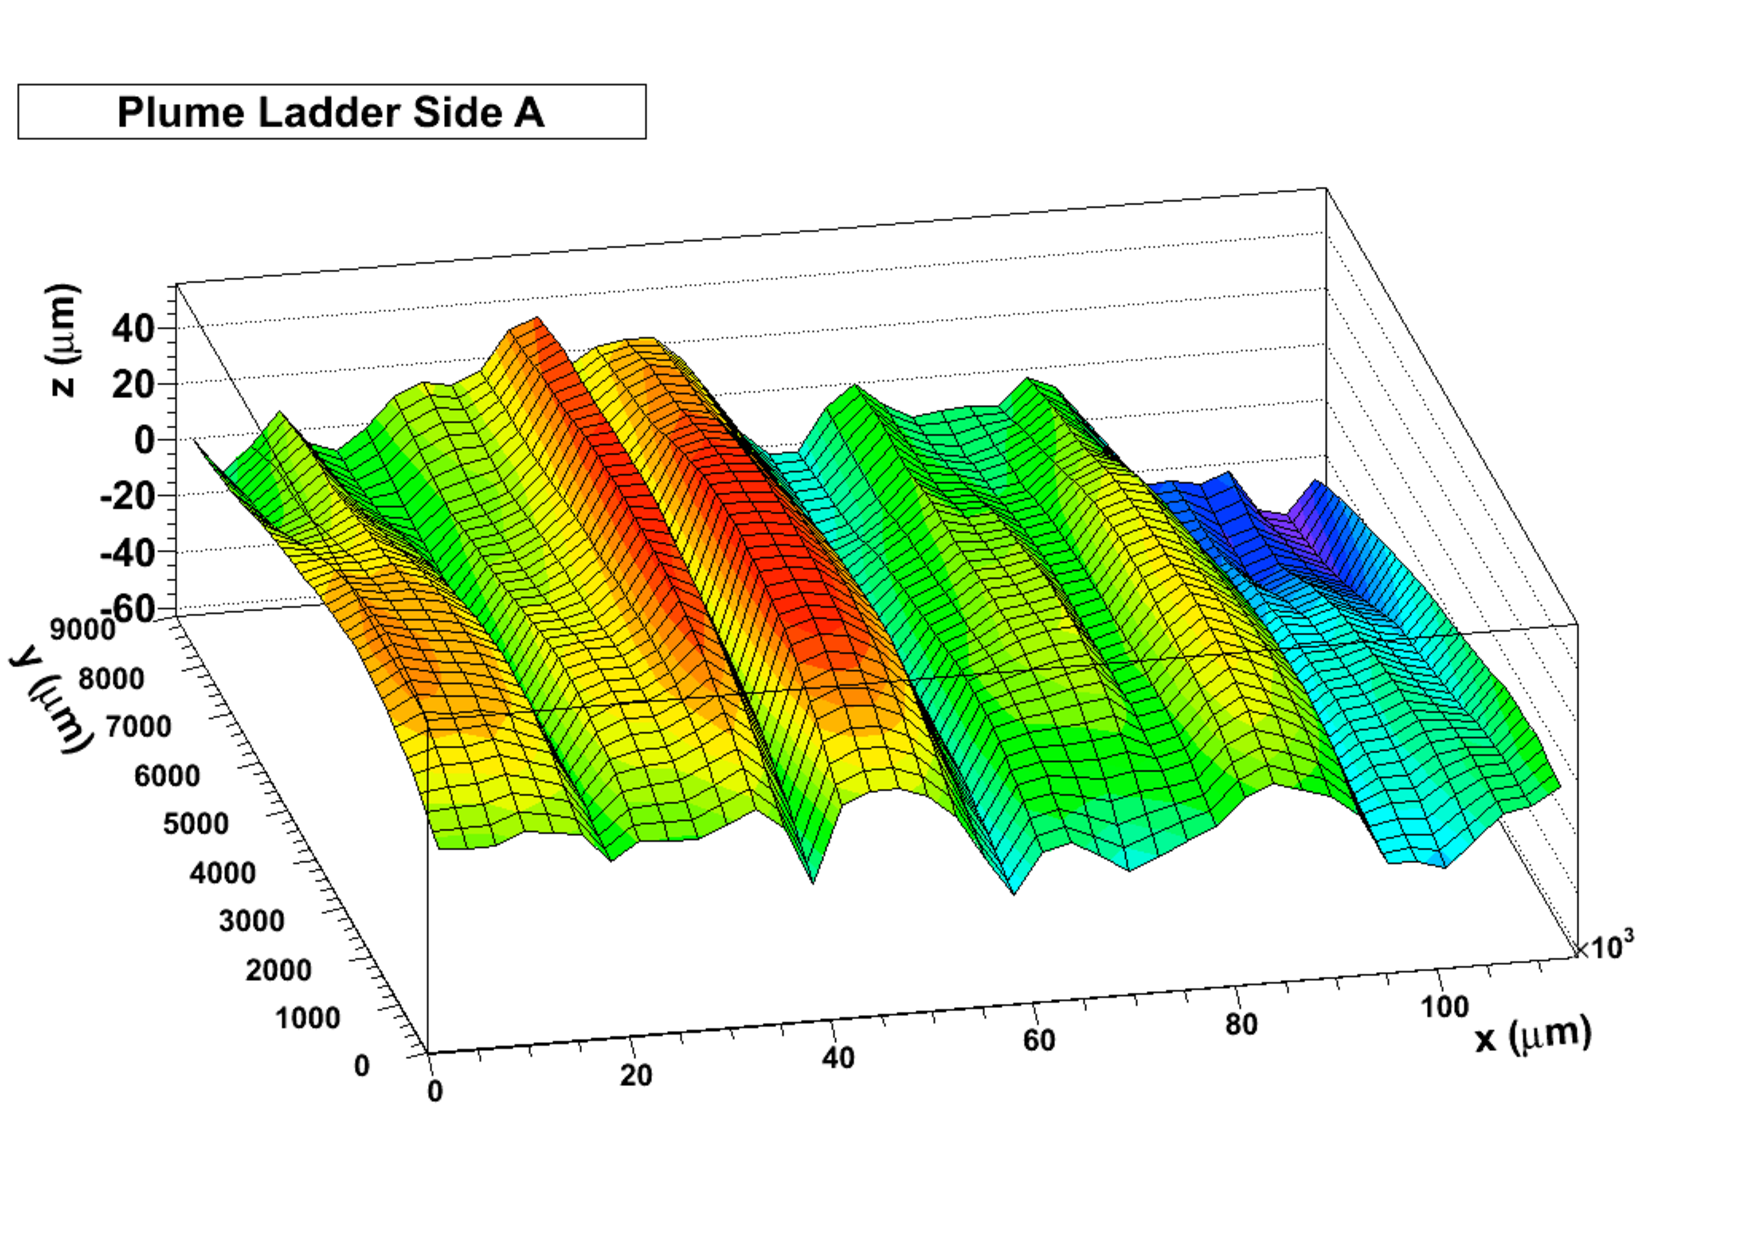
\includegraphics[width = 1.2\textwidth]{Pictures/deformation/surveyResults.pdf}
        \end{subfigure}
        \hfill
         %add desired spacing between images, e. g. ~, \quad, \qquad, \hfill etc. 
          %(or a blank line to force the subfigure onto a new line)
        \begin{subfigure}[t]{0.45\textwidth}
          \centering
          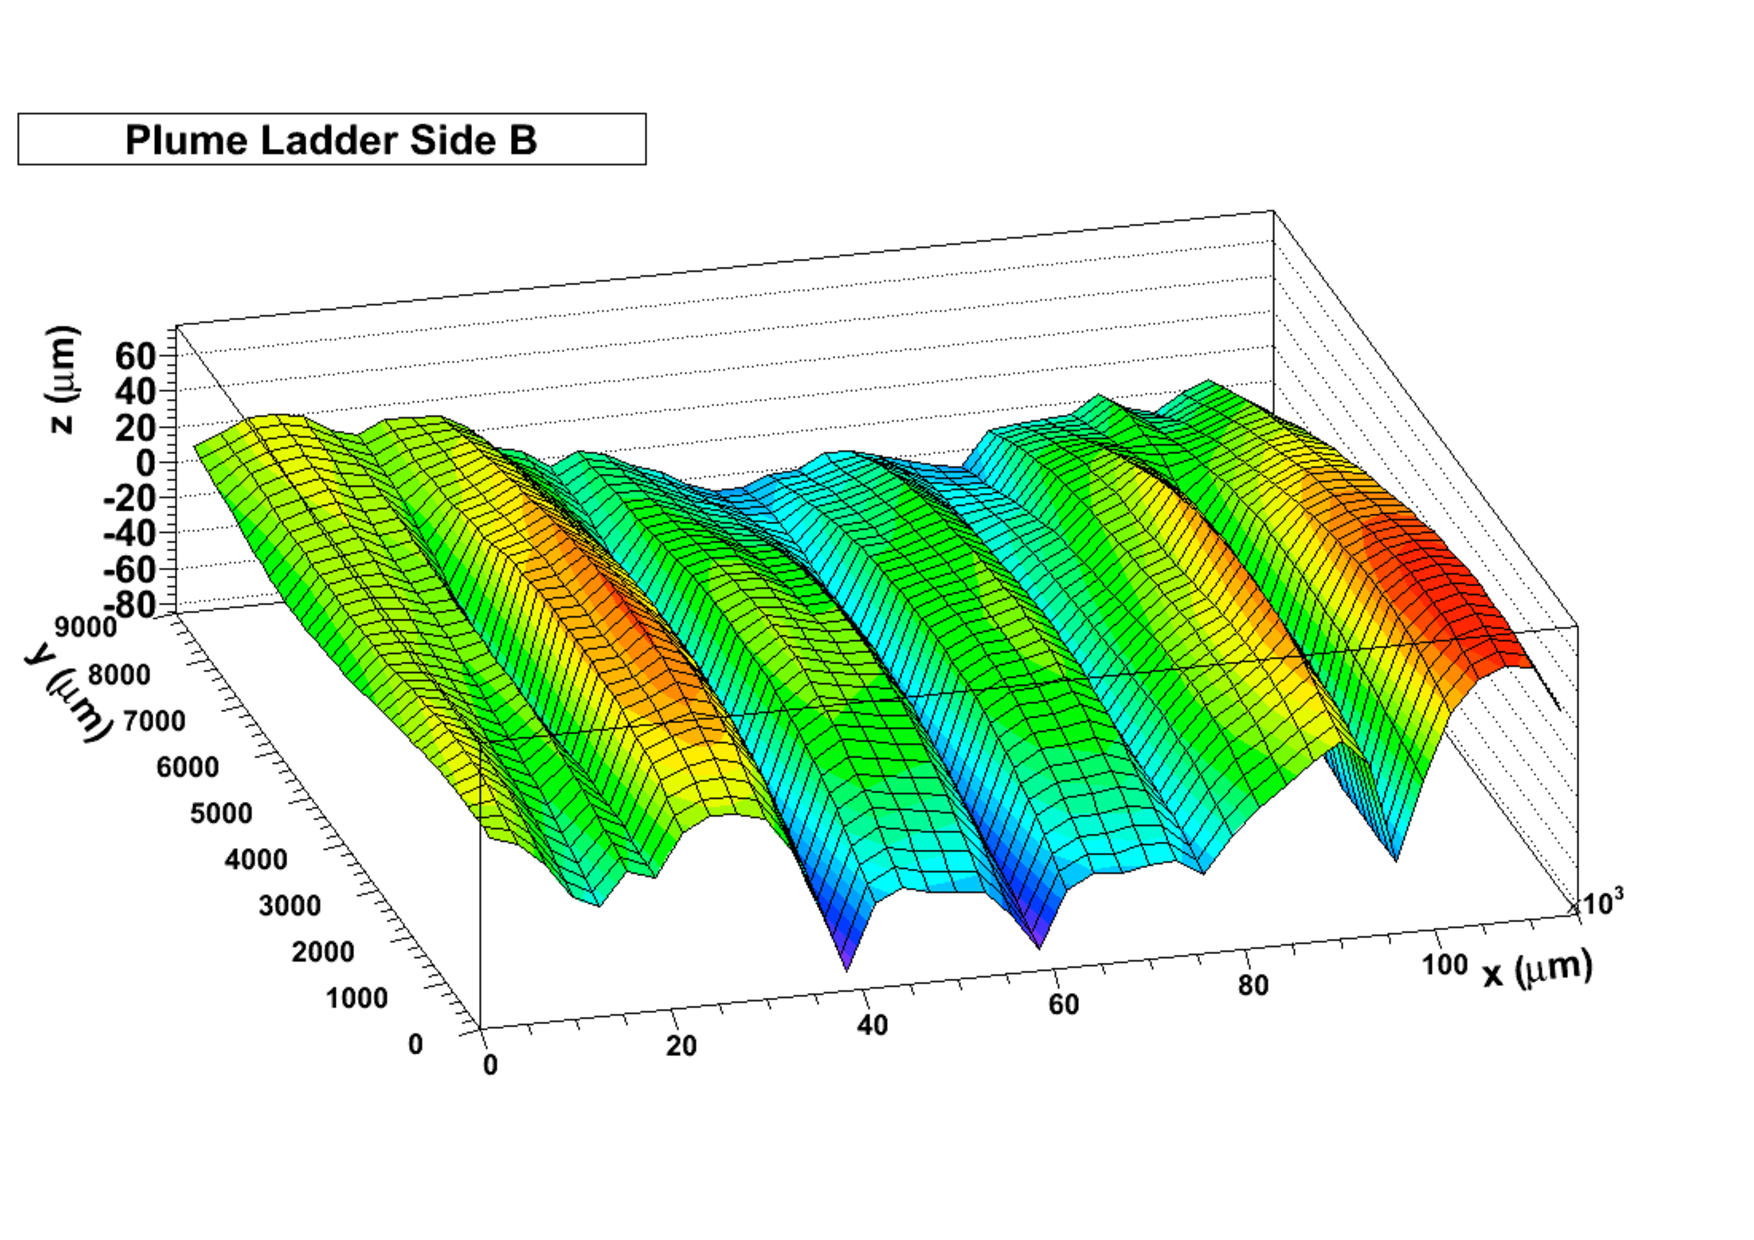
\includegraphics[width = 1.2\textwidth]{Pictures/deformation/surveyResultsB.pdf}
        \end{subfigure}

        \caption{Results of the mechanical survey of each side of the PLUME mechanical prototype.}
        \label{fig:mechanicalSurvey}
      \end{figure}

      A second origin of these deviations is due to the analysis.
      The sensors are modelled as completely flat planes and the $z$ position is fixed.
      However, the position in 3D of the sensor is actually different due to the deformations.
      When the particles are not hitting the sensor in normal incidence anymore, the hit predicted with respect to the flat plane does not have the same position anymore.
      Thus, the residual between the position of the extrapolated track and the predicted hit is increasing.
      As seen on the figure~\ref{fig:originDef}, the 

      \begin{figure}[!h]
      \centering
        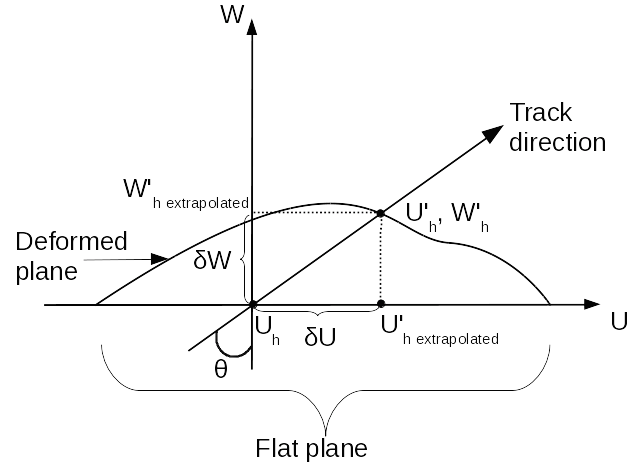
\includegraphics[width = 0.8\textwidth]{Pictures/deformation/origin_deformation.png}
        \caption{Side view of the sensor's deformation....}
        \label{fig:originDef}
      \end{figure}

      \subsubsection{Algorithm to estimate the deformations}

      A similar effect was observed in the CMS tracker during the alignment procedure with cosmic rays and a method was developed to compensate the deformations\cite{CMSalignment}. 
      By using Legendre polynomials to parametrise the sensors' deformation, they were able to minimise the deviations.
      The same methods was implemented in TAF.

      As tracks with a large angle of incidence are more sensitive to the exact position of the plane in 3 dimensions, the hits coordinates on the sensors have to be exactly known. 
      The information provided by the track-hit residuals deviations are related to the deformation behaviour. 
      To determine more precisely the hit position during the analysis, the deviations need to be used. 
      The distribution of the track-hit residuals as the function of the hit position is profiled and then fitted with a Legendre function. 
      Each coefficient given by the fit procedure are used to calculate the new hit position thanks to Legendre polynomials

      \begin{figure}
        %\centering
        \missingfigure{Residual after correction}
      \end{figure}
    
  \section{Benefits of double-sided measurement}

  %\todo{REF Loic thesis for TB@CERN results}
